%% ----------------------------------------------------------------
%% synopsis.tex -- MAIN FILE (the one that you compile with LaTeX)
%% ---------------------------------------------------------------- 

% Set up the document
\documentclass[a4paper, 12pt, twoside]{synopsis}  % Use the "synopsis" style, based on the ECS synopsis style by Steve Gunn
\graphicspath{{Figures/}}  % Location of the graphics files (set up for graphics to be in PDF format)

% Include any extra LaTeX packages required
\usepackage[square, numbers, comma, sort&compress]{natbib}  % Use the "Natbib" style for the references in the Bibliography
\usepackage{verbatim}  % Needed for the "comment" environment to make LaTeX comments
\usepackage{missing_packages/vector}  % Allows "\bvec{}" and "\buvec{}" for "blackboard" style bold vectors in maths
\usepackage{textcomp}
\usepackage{tikz}
\usepackage{setspace} 
\hypersetup{urlcolor=black, colorlinks=true}  % Colours hyperlinks in blue, but this can be distracting if there are many links.
\usepackage{times}
%\usepackage{missing_packages/lineno}
%\linenumbers
%% ----------------------------------------------------------------
\begin{document}
%\frontmatter	  % Begin Roman style (i, ii, iii, iv...) page numbering
% Set up the Title Page
\title  {Multi Segmented Image Transfer in Delay Tolerant Networks using Bandwidth Reduction Technique}
\authors  {\texorpdfstring
            {\href{pratyush.anand@st.com
}
            {Pratyush Anand}}
            {Pratyush Anand}
            }
\addresses  {\groupname\\\deptname\\\univname}  % Do not change this here, instead these must be set in the "synopsis.cls" file, please look through it instead
\date       {\today}
\subject    {}
\keywords   {}

\maketitle

%% ----------------------------------------------------------------

\setstretch{1.0}  % It is better to have smaller font and larger line spacing than the other way round

\pagestyle{plain}  % Return the page headers back to the "fancy" style

\setlength\parindent{20pt}

%% ----------------------------------------------------------------

\section{Introduction}
\indent Surveillance systems are ubiquitous and find many applications
in areas such as traffic monitoring, elderly care etc. Therefore, there
is a pressing need to evolve methods for conserving bandwidth while the
video data is transported from the point of acquisition to the point of
observation. Moreover, an increasing number of video sources rely on
resource constrained (bandwidth-limited, delay-tolerant) networks such
as Zigbee, DASH7 specially in smart home applications for the video
transport. With such networks at layer 1 and 2, there is a tremendous need
to conserve / preserve the bandwidth needed by each video stream / all
video streams collectively. We propose a method by which a few
pre-processing operations allow us to still carry out the primary
objective of surveillance while achieving large and impressive savings
on the required bandwidth.\\
\indent Video surveillance system can be integrated with existing home
network, but it is very important to achieve reduction in amount of
data to be transmitted due to lack of end to end connectivity. A low
data rate node also allows the system to remain in sleep mode for longer
durations and hence prolongs longer battery life.\\
\indent For surveillance data, only a few segments of image need to be
transmitted (the fast changing scenes).  Transmitting only significant
features pre-extracted locally from the image can reduce transmission
requirement significantly. However, this minimization of content must
allow reconstruction of the image with relevant details at the other
end. By extracting semantic information from deduced features, we reduce
the data rate even further. \\
\indent Automatic scene analysis, followed by extraction of desired
information can be complex, especially when application is targeted for
outdoor monitoring.  Sometimes background of the scene can be fast
changing, while in some other scene ambient light can be different.
Similarly, there can be many other hurdles in the process of automation.
But if an efficient background detection algorithm is chosen then, these
issues can be addressed. Further, the selected algorithm must allow
information extraction almost in real time. With latest research in
computer vision~\cite{9, 11}, it seems that such a task could be
viable with a low cost embedded system.\\
\section{Objective}
\indent	In this work we propose a solution for efficiently transforming
video data   over   a delay   tolerant   network.  We have addressed
the following problems in this work.\\
\begin{enumerate}
\item Evaluation of background subtraction algorithms (with reasonably
good result for surveillance applications) in terms of computational
complexity 
\item Evaluation of different techniques for moving object
skeletonization in terms of its suitability to calculate motion
descriptor feature 
\item Development of low computation algorithm to detect objects using
motion descriptor
\item Integration of proposed algorithm with low cost COTS embedded
hardware environment
\end{enumerate}
\section{Implementation}
\indent We have selected the Vibe~\cite{9} algorithm by Barnich et al.
for background subtraction, as it is computationally very efficient.
Since authors have not provided C code, we have developed our own C code
for this algorithm.\\
\indent Since surveillance object might be distant, so we have selected
skeleton motion approach for human detection. We have evaluated
different skeletonization methods and finally, the star skeletonization
method has been used~\cite{32}. Star skeletonization approach provides
an easy way for leg motion analysis. Analysis of leg motion allows us to
detect human from human, vehicle and animal. Since we have used
\textbf{Skel}etonized \textbf{M}otion \textbf{A}nalysis for object
detection, therefore we name our implementation as SKELMOT.\\
\indent All our code is either written from scratch or consists of other
code taken from public domain on a x86 based platform. We have coded in
C and on Linux platform. We did it so because C and Linux are widely
used with embedded platform.  Latest Linux kernel version also works
well for mmuless ARM core.  Therefore, it would be very easy to use same
code across wide range of micro-controllers and SOCs.\\
\indent It is also very important to benchmark the system which we are
using for test evaluation. However, none of the benchmark code provides
accurate figure for interpolation of results for any test. They are
considered for getting approximate benchmark. We benchmarked our x86
system with Dhrystone code.\\
\indent We have further evaluated performance of different
implementations on an ARM11 based system. We have used Raspberry Pi ,
which has a Broadcom BCM2835 system on a chip (SoC), that includes an
ARM1176JZF-S 700 MHz processor. We have also benchmarked this system
with Dhrystone code.
\section {Result Summary}
\indent We observe that with SKELMOT, we are able to detect a moving person
after a movement of three steps. Fig.  \ref{pipeline_images} shows output
images at different stages of the implementation.\\
\indent We have also done experiments with negative images like a person
moving on bicycle, or a vehicle moving on road. SKELMOT is successfully able
to discriminate between these objects. Fig. \ref{negative_inputs} shows
how it rejects moving vehicle and bicycle and  does not detect them as
human.\\
\begin{figure}[!t]
\centering
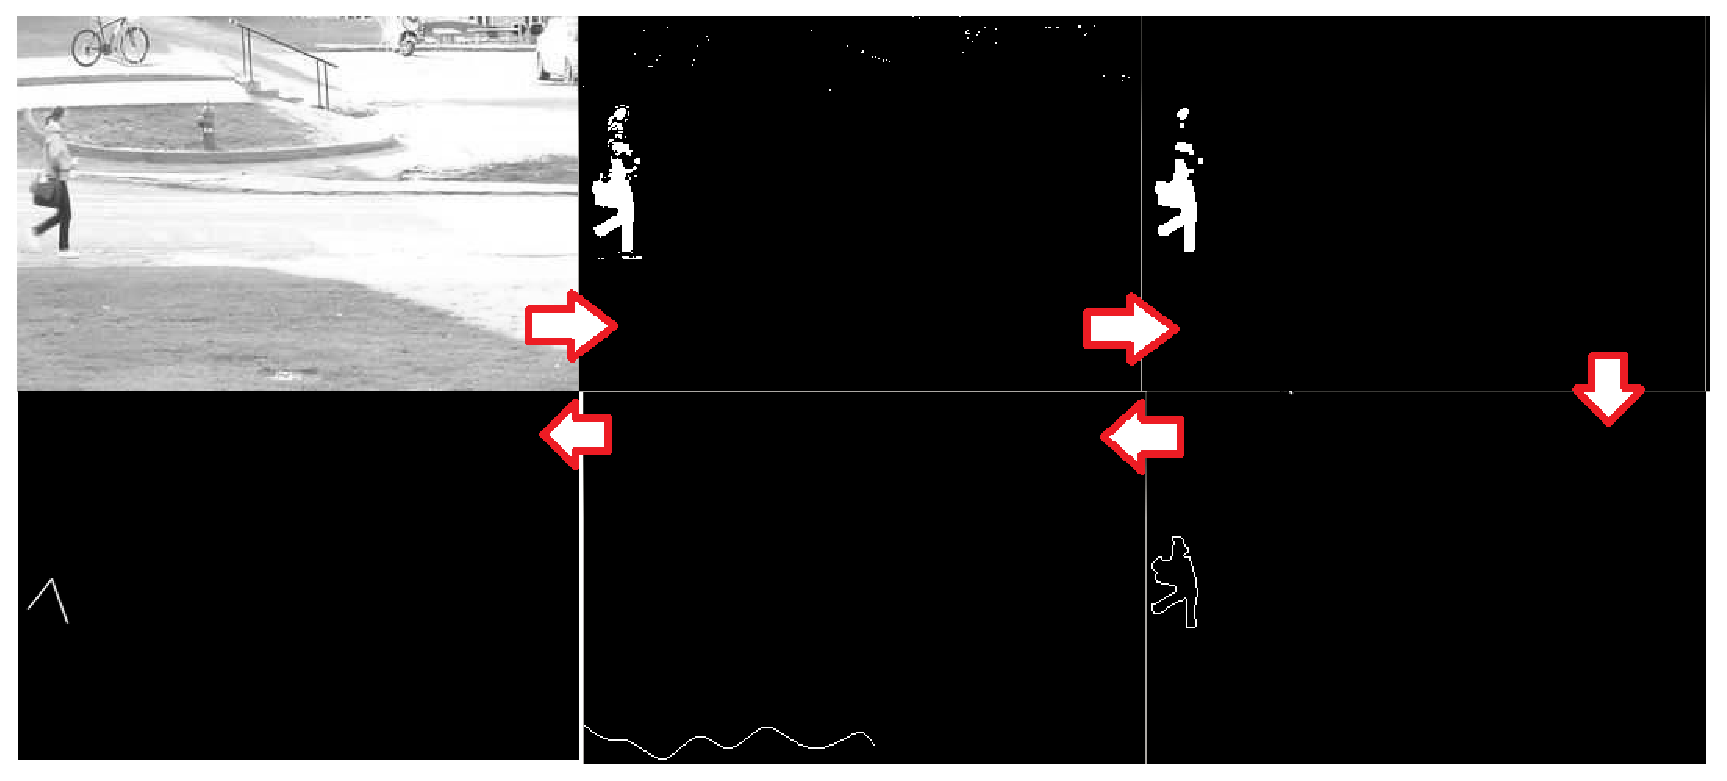
\includegraphics[scale=0.50]{Figures/pipeline_images}
\caption{Images at different stages of processing. (From top left in
	clockwise order)\\
	\textbf{(a)} Gray Scale input frame\\
	\textbf{(b)} Foreground extracted image using Vibe\\
	\textbf{(c)} Cleaned image\\
	\textbf{(d)} Contour of moving object\\
	\textbf{(e)} Plot of three points of interest, centroid and two distance
peaks nearer to bottom left and bottom right corner of bounding box\\
\textbf{(f)} Virtual representation of scene} 
\label{pipeline_images}
\end{figure}
\begin{figure}[!b]
\centering
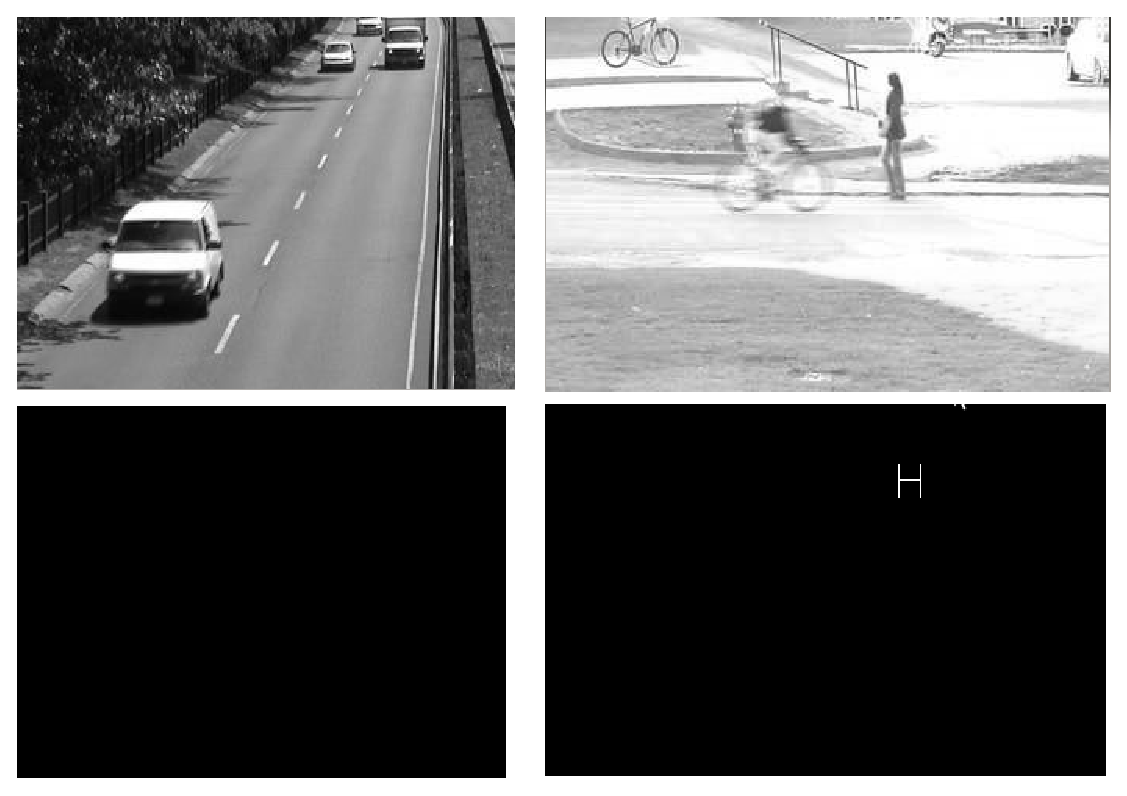
\includegraphics[scale=0.50]{Figures/negative_inputs}
\caption{Input and output in case of negative images}
\label{negative_inputs}
\end{figure}
\indent We have implemented and executed SKELMOT, Haar-like~\cite{17} and
covariance~\cite{19} feature based detection algorithm on both x86
desktop computer and embedded ARM platform. Comparison of execution time
has been shown in Fig.  \ref{pipeline_execution_time}. It shows a
definite improvement in execution speed of SKELMOT over Haar-like and
covariance feature based approach.  SKELMOT takes just 3.6 ms on the
average, while Haar-like and covariance feature based algorithm take
around 20 ms and 248 ms respectively per frame at x86 platform having
DMIPS = 800. Comparison of timing at ARM platform with DMIPS = 44 shows
that SKELMOT takes 182 ms on the average, while Haar-like and covariance
feature based algorithm take around 942 ms and 4.65 s respectively per
frame.  \\
\begin{figure}[!t]
\centering
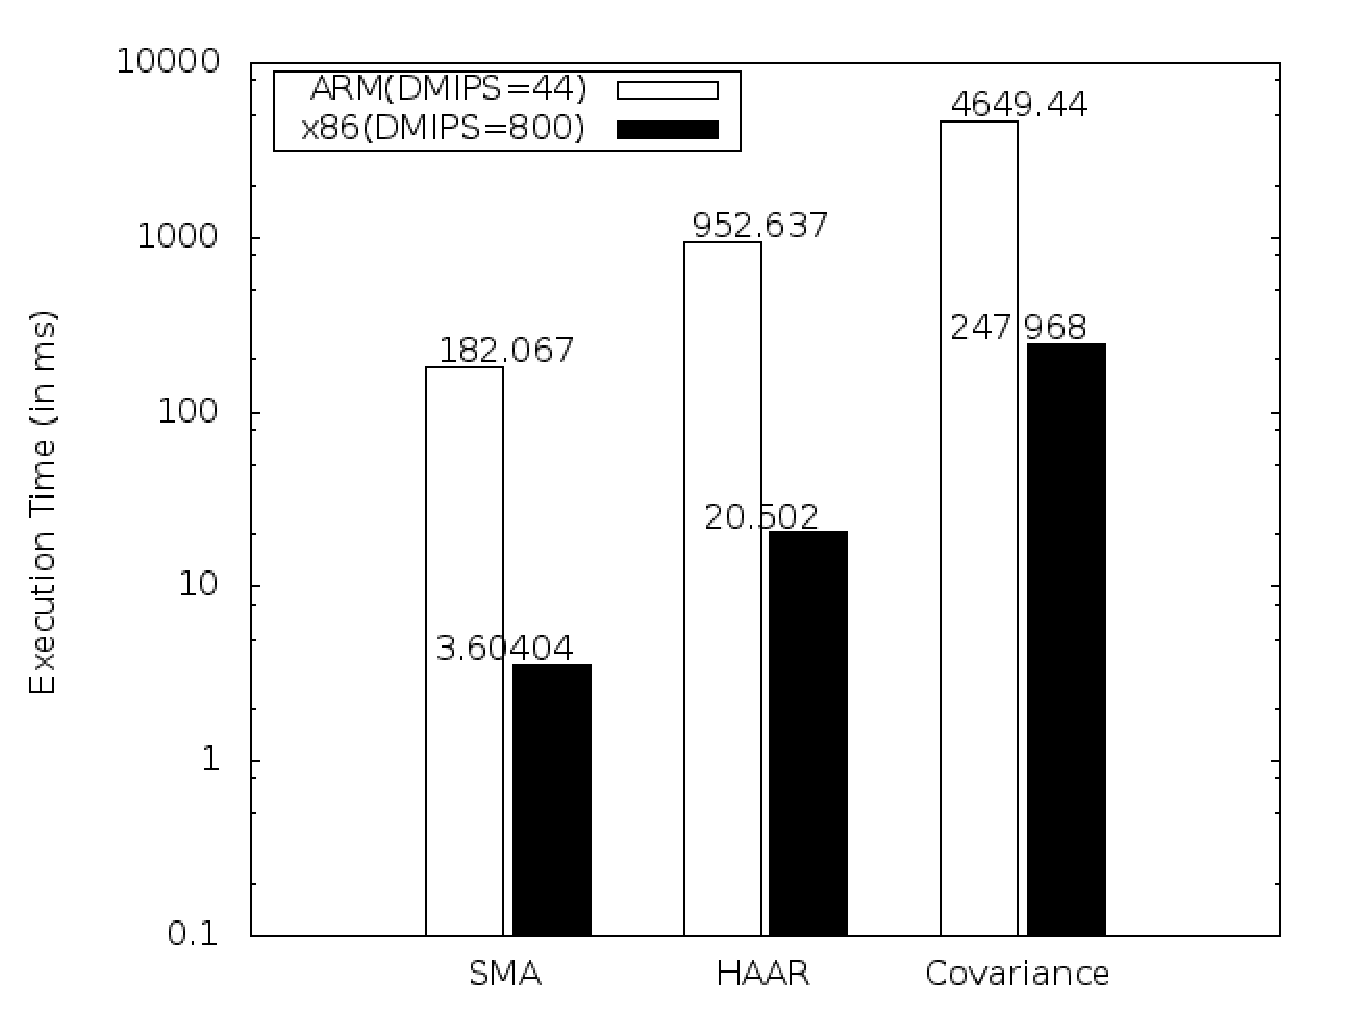
\includegraphics[scale=0.50]{Figures/pipeline_execution_time}
\caption{Execution time of evaluated algorithms with a ARM and x86
platform}
\label{pipeline_execution_time}
\end{figure}
\section {Publications}
\indent A paper titled ``Modifying Open Source Tools for Video
Pre-processing to achieve Ultra Low Bandwidth for Video Surveillance
over Delay Tolerant Networks`` has been communicated to the conference
"CERA 2013, IIT Roorkee" scheduled to be held between Oct. 3$^{rd}$ and
Oct. 5$^{th}$ 2013.\\
%% ----------------------------------------------------------------
  \clearpage

\label{Bibliography}
\addtotoc{Bibliography}
\lhead{\emph{Bibliography}}  % Change the left side page header to "Bibliography"
\bibliographystyle{ieeetr}  % Use the "unsrtnat" BibTeX style for formatting the Bibliography
%\bibliographystyle{apalike}
\bibliography{Bibliography}  % The references (bibliography) information are stored in the file named "Bibliography.bib"
\end{document}  % The End
%% ----------------------------------------------------------------
